\documentclass[]{report}
\usepackage{geometry}
\usepackage[utf8]{inputenc}
\usepackage{amsmath}
\usepackage{amsfonts}
\usepackage{amssymb}
\usepackage[pdftex]{graphicx}
\usepackage[space]{grffile}
\usepackage{epstopdf}
\usepackage{epsfig}
\usepackage{bmpsize}
\graphicspath{{./images/}}
\usepackage[export]{adjustbox}
\usepackage{wrapfig}
\usepackage{appendix}
\usepackage{listings}
\usepackage{hyperref}
\hypersetup{
	colorlinks=true,
	allcolors=blue,
	pdfborderstyle={/S/U/W 1}
}
\usepackage{hypcap}

\begin{document}

\title{iCampus Development}
\author{James Antrim, Mariusz Homeniuk, Kristijan Pokas, Wolf Rost, Niklas Simonis}

\begin{figure}

\includegraphics[width=14cm]{thm.png}
\maketitle
\end{figure}

\newpage
\tableofcontents

\chapter{Introduction}

This documents explains how to set up and develop in the context of the iCampus Working Group. All instructions in this document are based upon the Windows 8.1 operating system.

\chapter{The Development Environment}

In order to develop on a personal computer, must certain steps be performed in various systems, as well as various programs installed and configured. In this chapter these items will be discussed.

\section{Local Web Server Installation and Configuration}

In order for a locally developed project to be deployed, and to guarantee access to all required components a web server must be installed locally. 

\subsection{XAMPP}

In the iCampus web development group we use XAMPP from Apache Friends for our local web servers. Apache Friends describes XAMPP as follows:

\begin{quote}
	\textit{XAMPP is a completely free, easy to install Apache distribution containing MySQL, PHP, and Perl. The XAMPP open source package has been set up to be incredibly easy to install and to use.}\footnote{\url{https://www.apachefriends.org/index.html} September 19, 2014}
\end{quote}

\noindent
As per the description the distributions of XAMPP available from \href{https://www.apachefriends.org/index.html}{Apache Friends} come included with various useful tools which are also used within iCampus, such as PHP (server-side scripting language)abd MySQL (database management system), as well as many other tools which are optional for iCampus such as FileZilla (FTP Server) and Mercury (Mail Server).\\
\\
Download and install the latest XAMPP installation. Keeping in mind that at least MySQL and phpMyAdmin need to be installed to function in the iCampus environment.

\begin{figure}[h] 
	\centering
	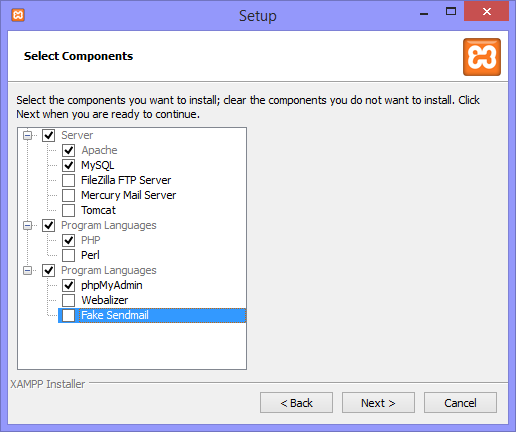
\includegraphics[width=6cm]{xampp.png}
	\caption{XAMPP Minimum Installation}
\end{figure}

\newpage
\subsection{PHP Configuration}
\label{subsec:phpconfig}

The next step is the configuration of PHP for error reporting using xdebug. To do this open your php.ini file using the XAMPP control panel or the file explorer. This file is typically located at \url{C:/xampp/php/php.ini}.\\

\begin{figure}[h] 
	\centering
	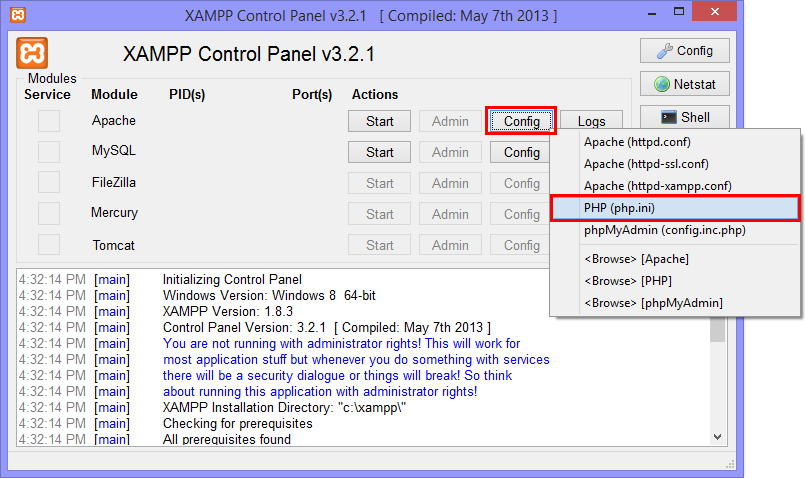
\includegraphics[width=6cm]{openphpini.png}
	\caption{XAMPP Control Panel}
	\label{fig:xamppcontrolpanel}
\end{figure}

The following modifications should then be made to the file:\\
\\

\begin{tabular}{l}
// Reports all PHP Errors, Warnings, and Breaches of PHP Standards\\
\texttt{error\_reporting = E\_ALL | E\_STRICT}\\\\

// Turns off error buffering =$>$ errors reported immediately, necessary for the debugger\\
\texttt{output\_buffering = Off} \\\\
\end{tabular}

\begin{tabular}{l}
// Debugger Settings (may only need to be commented in)\\
\texttt{[XDebug]} \\
\texttt{zend\_extension="C:\textbackslash xampp\textbackslash php\textbackslash ext\textbackslash php\_xdebug.dll"}\\
\texttt{xdebug.remote\_enable=true}\\
\texttt{xdebug.remote\_host=localhost}\\
\texttt{xdebug.remote\_port=9000}\\
\texttt{xdebug.remote\_handler=dbgp}\\
\texttt{xdebug.profiler\_enable=1}\\
\texttt{xdebug.profiler\_output\_dir="C:\textbackslash xampp\textbackslash tmp"}\\\\
\end{tabular}

\noindent
The interface shown in Figure \ref{fig:xamppcontrolpanel} above will also later used to start and stop the server service itself, Apache, as well as the the supporting database management service, MySQL, by pressing the corresponding ``Start"/``Stop" button.

\subsection{PEAR Configuration}

In order to eliminate possible error sources, PEAR must next be configured. To this end run cmd.exe as an administrator and execute the following commands.\\

\begin{tabular}{l}
// Navigate to the PHP Directory\\
\texttt{cd C:\textbackslash xampp\textbackslash php}\\
\\
// Display the PEAR Configuration\\
\texttt{pear config-show} \\
\\
\end{tabular} 

\subsubsection{Directory Configuration}

The following settings which may refer to C:\textbackslash php\textbackslash pear need to be changed to point to C:\textbackslash xampp\textbackslash php\textbackslash pear should they not already do so.\\

\begin{tabular}{l}
\texttt{pear config-set doc\_dir C:\textbackslash xampp\textbackslash php\textbackslash pear\textbackslash docs} \\
\texttt{pear config-set cfg\_dir C:\textbackslash xampp\textbackslash php\textbackslash pear\textbackslash cfg} \\
\texttt{pear config-set data\_dir C:\textbackslash xampp\textbackslash php\textbackslash pear\textbackslash data} \\
\texttt{pear config-set cache\_dir C:\textbackslash xampp\textbackslash php\textbackslash pear\textbackslash cache} \\
\texttt{pear config-set download\_dir C:\textbackslash xampp\textbackslash php\textbackslash pear\textbackslash download} \\
\texttt{pear config-set temp\_dir C:\textbackslash xampp\textbackslash php\textbackslash pear\textbackslash temp} \\
\texttt{pear config-set test\_dir C:\textbackslash xampp\textbackslash php\textbackslash pear\textbackslash tests} \\
\texttt{pear config-set www\_dir C:\textbackslash xampp\textbackslash php\textbackslash pear\textbackslash www} \\
\texttt{pear config-set php\_ini C:\textbackslash xampp\textbackslash php\textbackslash php.ini}
\end{tabular}

\newpage
\subsubsection{Channel Configuration}

Next PEAR itself and its channel list needs to be updated, so that later updates for extensions can be automatically pulled from their respective channels. Thereafter the auto\_discover variable is set to on, this allows new channels to be discovered and dependencies to be resolved automatically.\\


\begin{tabular}{l}
// Ensures the latest PEAR version\\
\texttt{pear upgrade pear}\\
\\
// Empties the PEAR Cache\\
\texttt{pear clear-cache}\\
\\
// Turns on Automatic Discovery\\
\texttt{pear config-set auto\_discover 1}\\
\\
// Discover and Add the pear.phpunit.de Channel (usually already present)\\
\texttt{pear channel-discover pear.phpunit.de}\\
\\
// Update the Channel list\\
\texttt{pear update-channels}\\
\\
// Uninstalls CodeSniffer in Case a Deprecated Version is Present\\
\texttt{pear uninstall PHP\_CodeSniffer}\\
\\
// Installs PHP CodeSniffer\\
\texttt{pear install PHP\_CodeSniffer}\\
\\
// Discovers the PHP Mess Detector channel\\
\texttt{pear channel-discover pear.phpmd.org}\\
\\
// Lists available packages\\
\texttt{pear remote-list -c phpmd}\\
\\
// Installs PHP Mess Detector Package 1.5.0, actual as of 27 Sept, 2014\\
\texttt{pear install phpmd/PHP\_PMD-1.5.0}\\ \\
\end{tabular}

\noindent
More about Code Sniffer and Mess Detector in Section \ref{sec:qatools}.

\newpage

\section{Git}

For repository and versioning iCampus uses Git. To this end Git must first be downloaded from \href{http://git-scm.com/downloads}{Git}, installed and configured.

\subsection{Installation}

\subsubsection{Command Context}
Part of the configuration is deciding which context you would like to be able to use Git in. In iCampus the second is used because it allows the developer later to use PHPStorm's own terminal to execute Git's commands, which eliminates the necessity for navigation to projects in Git Bash or Windows shell. More on PHPStorm in Section \ref{sec:PHP-Storm}.\\

\begin{figure}[h] 
  \centering
     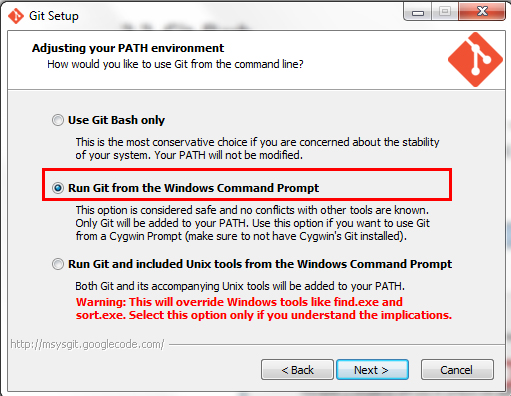
\includegraphics[width=6cm]{gitbash1.jpg}
  \caption{Command Context}
\end{figure}

\subsubsection{Line Endings}

The next screen lets one decide how file endings are pulled and committed. The iCampus Coding standards demand the Unix-style line endings. To this end only the second option is sufficient, because once style checking is enabled in your IDE the first and third options will, dependent on your system settings, report every single line of code as a breach of style, which removes any transparency whatsoever when searching for other errors.\\

\begin{figure}[h] 
  \centering
     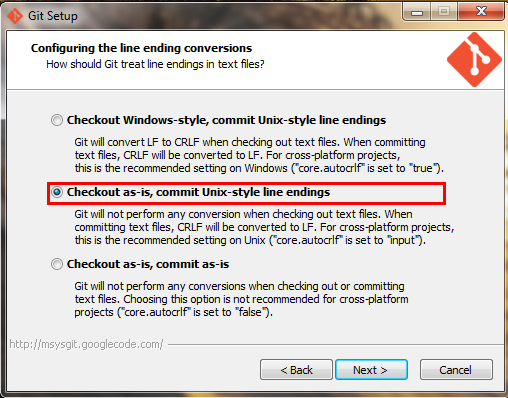
\includegraphics[width=6cm]{gitbash2.jpg}
  \caption{Line Endings}
\end{figure}

\subsection{User Configuration}

In order to take part in the development process you must take several steps to configure your user account.

\subsubsection{Global User Configuration}
In Git Bash the global user name and email must be set so that repository actions can be associated with a user.\\
\\
Start Git Bash and enter the following commands, replacing $<$First Name$>$, $<$Last Name$>$, and $<$Department$>$ with your first and last names and the abbreviation of the department in which you are matriculated.\\
\\
\begin{tabular}{l}
\texttt{git config --global user.name "$<$First Name$>$ $<$Last Name$>$"}\\
\texttt{git config --global user.email "$<$First Name$>$.$<$Last Name$>$@$<$Department$>$.thm.de"}\\
\end{tabular}\\
\\
You can confirm that the entries were saved correctly by entering the following command and comparing the associated values.\\
\\
\begin{tabular}{l}
\texttt{git config -l}
\end{tabular}

\subsubsection{SSH-Key Creation}

After the user configuration is completed, an SSH-Key can be created using the following command in Git Bash.\\
\\ 
\texttt{ssh-keygen}\\
\\
The first question determines where the generated key will be saved and what its name will be. Per default this will be \textbf{\texttt{C:/Users/$<$Windows Account Name$>$/.ssh/id\_rsa}}. This directory is important for the next steps, as well as later when repositories are cloned. Press enter to confirm the default.
The next two questions will be to enter and confirm your password. You can also elect to have no password by pressing enter in answer to both questions.

\subsubsection{SSH-Key in Gitorious eintragen}

The freshly created key must now be added to the repository server in order to associate you as a user to projects for which you have access. First visit \url{http://scm.thm.de} and log in. After this your username will appear in the upper right hand corner between the search field and a button with a white arrow on it. Click on the arrow and select \texttt{Settings}.\\
\\
\begin{figure}[h] 
  \centering
     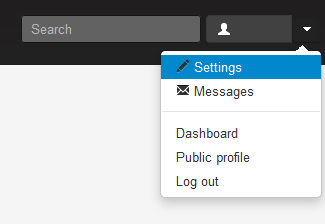
\includegraphics[width=5cm]{gitorious1.jpg}
  \caption{Settings Selection}
\end{figure}

\noindent
Here we need to select the fourth tab \texttt{SSH Keys} and add the key using the \texttt{Add new} button.\\

\begin{figure}[h] 
  \centering
     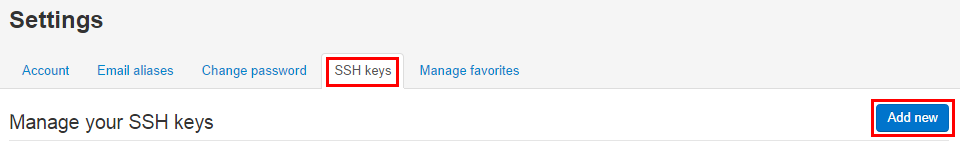
\includegraphics[width=10cm]{gitsettings.png}
  \caption{Settings Navigation}
\end{figure}

\noindent
In the form that opens we have to copy the text of the public key. This can be found in the directory created during the creation of the key, \texttt{C:/Users/$<$Windows Account Name$>$/.ssh/id\_rsa.pub}. Open this file with a text editor, copy the text from the file, and paste it into the available text field. At the end of the pasted text will be a \texttt{$<$Name$>$@$<$Domain$>$}. This should be replaced with the email address from the Git Configuration. When this has been completed click the \texttt{Save} button.

\newpage

\section{PhpStorm}
\label{sec:PHP-Storm}

PhpStorm is the IDE used in iCampus. While others are allowed the use of a single IDE in the working group allows for the exchange of information and tips on how to get the most out of a single IDE. This makes everyone more productive and allows for a collaborative effort to solve any problems which may be IDE related.\\
\\
PhpStorm was chosen for its ease of use and integration of many tools which simplify development, including CodeSniffer, database connection tools, SASS support, Git support, and many others. PhpStorm can be downloaded from the \href{http://www.jetbrains.com/phpstorm/}{JetBrains Website}.

\subsection{Installation}
During the installation process you will be asked which file extensions should be associated with PhpStorm. As we use PhpStorm for the development with all given extensions, all can be selected. As of PhpStorm 8 this also allows for the editing of single files without the creation of a project.\\

\begin{figure}[h] 
  \centering
     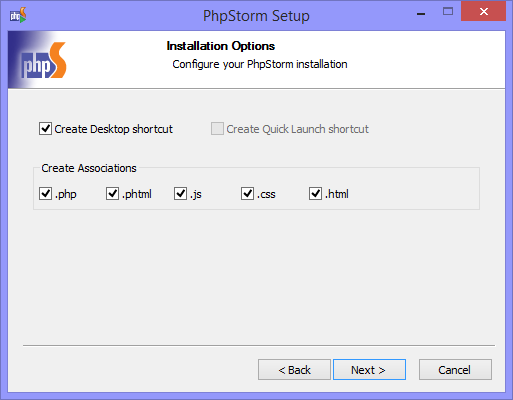
\includegraphics[width=5cm]{fileassociations.png}
  \caption{File Associations}
\end{figure}

\noindent
For the most part the rest of the installation requires nothing special, however at the end you will be asked to chose between several themes and coloring/font style options. As this interface offers no preview it is best to go with the default settings. These selections can later be changed while running the PhpStorm which will actually show you what effects your selection has on its appearance.\\
\\
After the installation starting PhpStorm will start the activation dialog. Here you will need to enter a ``User or Company Name" and a ``License Key". The name for our license is \texttt{Technische Hochschule Mittelhessen - University of Applied Sciences}. The license key will be given to you directly.

\newpage

\begin{figure}[h] 
	\centering
	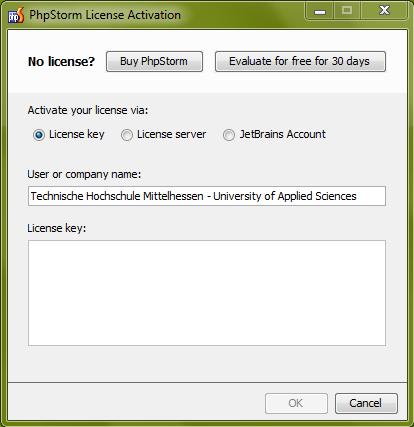
\includegraphics[width=6cm]{phpstormactivation.png}
	\caption{PhpStorm License Activation}
\end{figure}

\subsection{THM Core Library}

Next both for example and the inherent utility of the library we will create the project \texttt{lib\_thm\_core} by cloning the respository and checking out the development branch. Start PhpStorm and select \texttt{Check out from Version Control} from the ``Quick Start" area and \texttt{Git} from the drop-down menu that appears. \texttt{Check out from Version Control} can later be reached under the \texttt{VCS} main menu entry.

\begin{figure}[h] 
	\centering
	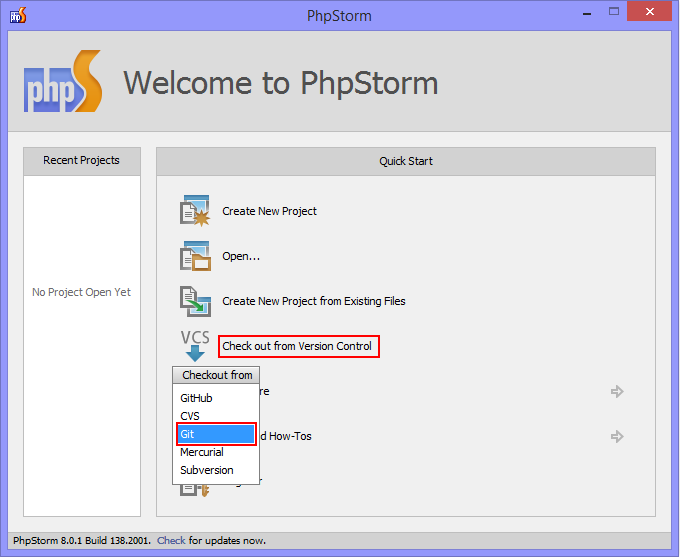
\includegraphics[width=6cm]{newprojectfromgit.png}
	\caption{Check out a Git Project}
\end{figure}

\noindent
We will want to use \texttt{git@scm.thm.de:icampus/lib\_thm\_core.git} as the ``Git Repository Url". At this point PhpStorm will complain that the PhpstormProjects directory does not exist. Either create the default directory at the location shown or chose a different directory into which this (and your future projects if you so chose) will be saved.\\
\\
\begin{figure}[h] 
	\centering
	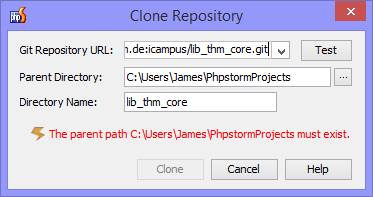
\includegraphics[width=5cm]{clonerepositoryerror.png}
	\caption{Clone Repository}
\end{figure}

\noindent
While checking out you will be asked if you wish to save the server's SSH key to your list of known hosts, click ok to continue. You will then be asked if you would like to open the project you just created, click yes.\\
\\
Since we did not include the branch name while cloning the repository, you will have checked out the master branch. In iCampus, with few very specific exceptions, \textbf{no one should be developing in the master branch}, for this reason we will now check out the development branch. This can be accessed in at least three ways. The way I find easiest is the branch display in the lower right hand corner. Click on the branch display, then the branch to be checked out, \texttt{origin/development}, and then \texttt{Checkout as a new local branch}.\\
\\
\begin{figure}[h] 
	\centering
	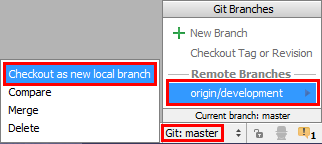
\includegraphics[width=5cm]{checkoutbranch.png}
	\caption{Branch Checkout}
	\vspace{-15pt}
\end{figure}

\newpage

\section{Code Sniffer and Mess Detector}
\label{sec:qatools}

Now that we have checked out \texttt{lib\_thm\_core}, we can use the coding standards within it to set up PHP CodeSniffer.

\begin{quote}
	PHP\_CodeSniffer is a PHP5 script that tokenises and ``sniffs" PHP, JavaScript and CSS files to detect violations of a defined coding standard. It is an essential development tool that ensures your code remains clean and consistent. It can also help prevent some common semantic errors made by developers.\footnote{\url{http://pear.php.net/manual/en/package.php.php-codesniffer.intro.php} Stand September 22, 2014}
\end{quote}

\noindent
PHP Mess Detector on the other hand searches for problems more abstract and more serious such as\footnote{\url{http://phpmd.org/} Stand September 27, 2014}:

\begin{itemize}
	\item Possible bugs
	\item Suboptimal code
	\item Overcomplicated expressions
	\item Unused parameters, methods, properties
\end{itemize}

\subsection{Standards Directory Inclusion}

First we will create symbolic links from the Joomla and THMJoomla folders to the folder which holds the existing standards. Open the windows shell as administrator and enter the following in the form \texttt{Command Link Target}.\\
\\
\textbf{Joomla Standard}
\begin{description}
	\itemsep-10pt
	\item[Command] \texttt{mklink /d}\\
	\item[Link] \texttt{C:\textbackslash xampp\textbackslash php\textbackslash pear\textbackslash PHP\textbackslash CodeSniffer\textbackslash Standards\textbackslash Joomla}\\
	\item[Target] \texttt{C:\textbackslash $<$System Specific Path$>$\textbackslash lib\_thm\_core\textbackslash coding\_standards\textbackslash Joomla}\\
\end{description}

\noindent
\textbf{iCampus Standard}
\begin{description}
	\itemsep-10pt
	\item[Command] \texttt{mklink /d}\\
	\item[Link] \texttt{C:\textbackslash xampp\textbackslash php\textbackslash pear\textbackslash PHP\textbackslash CodeSniffer\textbackslash Standards\textbackslash THMJoomla}\\
	\item[Target] \texttt{C:\textbackslash $<$System Specific Path$>$\textbackslash lib\_thm\_core\textbackslash coding\_standards\textbackslash THMJoomla}\\
\end{description}

\newpage

\subsection{PhpStorm}

In order for Code Sniffer and Mess Detector to perform in PhpStorm they must first be integrated. This can be set as part of the default settings, meaning the settings will be applied to all projects, or in the project settings, where they would only valid for a specific project. The steps are exactly the same, but the entry point is slightly different. First access the settings using the menu item \texttt{File} and then selecting either \texttt{Default Settings...} or \texttt{Settings...} from the drop down menu.

\subsubsection{PhpStorm Inclusion}

To activate Code Sniffer click on \texttt{PHP} and then \texttt{Code Sniffer} or \texttt{Mess Detector}. In the text field next to ``PHP Code Sniffer (phpcs) path" enter the path to phpcs.bat. In the standard installation this will be \texttt{C:\textbackslash xampp\textbackslash php\textbackslash phpcs.bat}. After you have input the path, click on \texttt{Validate}. If the file is valid, the you will be shown a short text containing the version of the installed Code Sniffer. Although not specifically stated the steps for Mess Detector inclusion are completely analogous.\\
\\
\begin{figure}[h] 
	\centering
	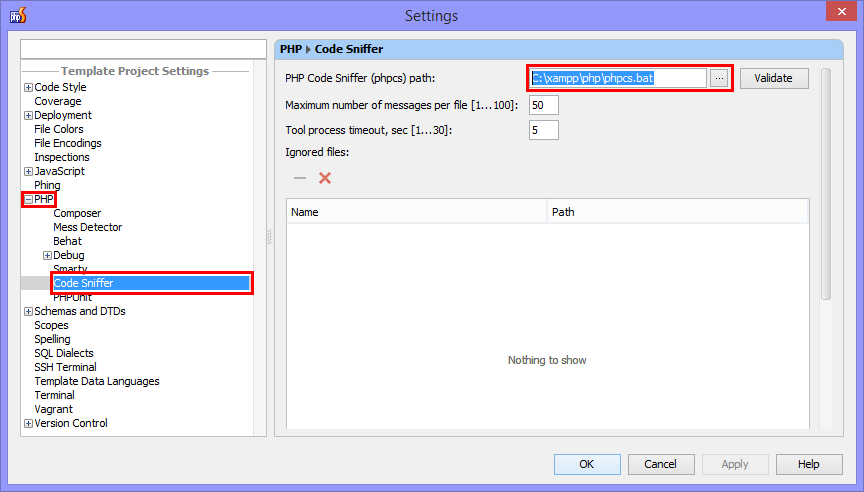
\includegraphics[width=14cm]{codesnifferinclusion.png}
	\caption{Code Sniffer - PhpStorm Inclusion}
\end{figure}

\subsubsection{PhpStorm Configuration}

Next we need to add PHP\_CodeSniffer to the inspections performed. With the settings still open, click on \texttt{Inspections}, then in the list to the right \texttt{PHP}, and finally on \texttt{PHP Code Sniffer validation} to open the configuration settings for Code Sniffer.\\
\\
\begin{figure}[h] 
	\centering
	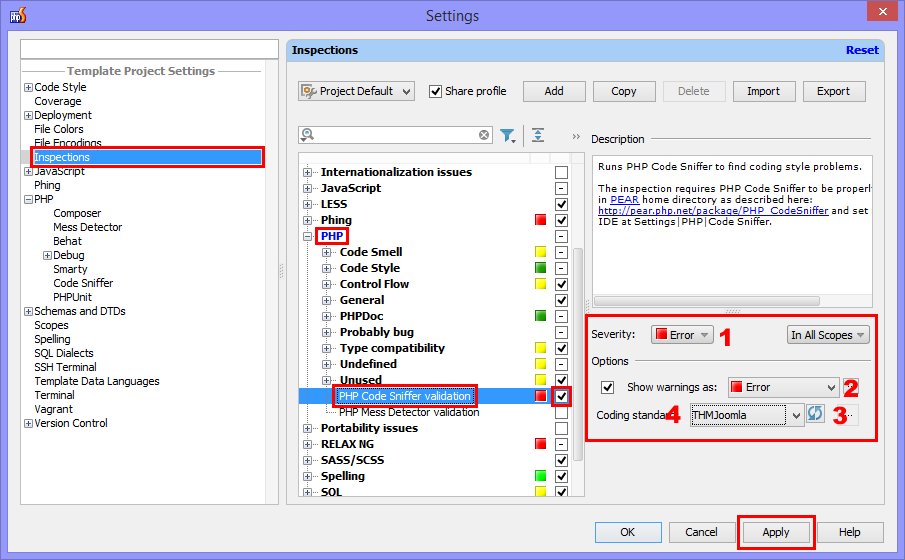
\includegraphics[width=14cm]{codesnifferconfiguration.png}
	\caption{Code Sniffer - PhpStorm Configuration}
	\label{fig:cspsc}
\end{figure}

\noindent
To activate the inspection we must first set the checkbox next to \texttt{PHP Code Sniffer validation}. This activation enables the further settings to the right which we see numbered with one through four in Figure \ref{fig:cspsc}.

\begin{enumerate}
	\item \texttt{Inspection severity}:``indicates how seriously the code issues detected by the inspection impact the project and determines how the detected issues should be highlighted in the editor."\footnote{http://www.jetbrains.com/phpstorm/webhelp/configuring-inspection-severities.html Stand September 22, 2014}
	\item \texttt{Display severity}: defines how the infractions found are marked.
	\item \texttt{Refresh}: updates the list of available coding standards. Should the desired standard not be found in the folder defined in the section on symbolic links, you can also manually search for the standard on your file system.
	\item \texttt{Available standards}: a list of standards found. In iCampus we use the THM Joomla Standard which inherits or extends many of the definitions in the Joomla standard.
\end{enumerate}

\noindent
It is recommended that both inspection and display severity be set to errors to make the standard infractions more noticable. Settings take effect when the \texttt{Apply} button has been pressed.\\
\\
Inspection settings for Mess Detector are also analogous here, with the distinction that one need not select a standard, instead selecting which rule sets should be applied.

\newpage
\section{SASS}

In iCampus we strive to maintain a standardized appearance both within views of the same extension as well as between extensions developed by the iCampus Group as a whole. To this end we utilize SASS.

\begin{quote}
	Sass is an extension of CSS that adds power and elegance to the basic language. It allows you to use variables, nested rules, mixins, inline imports, and more, all with a fully CSS-compatible syntax. Sass helps keep large stylesheets well-organized, and get small stylesheets up and running quickly, particularly with the help of the Compass style library.\footnote{\url{http://sass-lang.com/documentation/file.SASS_REFERENCE.html} Stand 27 September, 2014}
\end{quote}

The above mentioned variables, nested rules, mixins, and inline imports allow the centralization of style structures and recurring themes, while still allowing for individualized style elements as required.\\
\\
In iCampus we use the SCSS SASS syntax which closely resembles most .css you will have seen, and, stand alone, are actually valid CSS3 documents. This has as a consequence that our SASS files developed later will actually end with the extension .scss. For more information read \href{http://sass-lang.com/documentation/file.SASS_REFERENCE.html#syntax}{the SASS syntax explanation}.

\subsection{Installation}

Logically SASS must first be installed on the local system in order to function. This in turn requires the Ruby programming language, for which sass and compass are packages. While we need Ruby on the local system for SASS to function, we will not be using it to program, for this reason only the minimal requirements as pertain to SASS installation will be discussed.\\
\\
Ruby can be installed by visiting \href{http://www.rubyinstaller.org/downloads/}{the ruby installer downloads page} and choosing the download that best suits your operating systems needs, as described in the right hand column.\footnote{Stand 27 September, 2014}\\
\\
After you have downloaded and started the Ruby installation executable and accepted the license agreement you will be confronted with choices regarding the installation directory, support features, path variables, and file associations. We recommend using the default file path as it makes finding the installation easier, should any problems arise. You should only choose to install Td/Tk support if you know that you will be developing GUI applications in Ruby. The path variable is required in order for SASS to function. The association of .rb and .rbw files with this installation is recommended.

\newpage

\begin{figure}[h] 
	\centering
	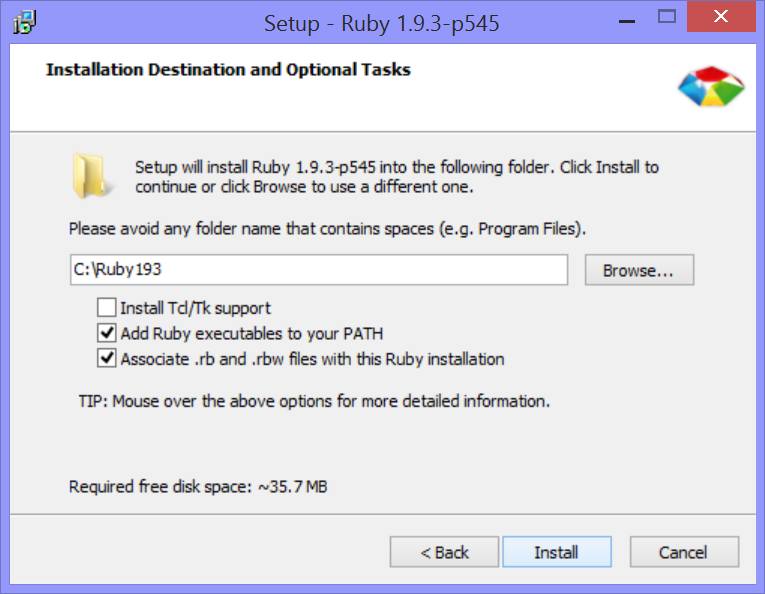
\includegraphics[width=5cm]{rubyinstallation.png}
	\caption{Ruby Installation}
	\label{fig:rubyinstallation}
\end{figure}

\noindent
After ruby is installed we can begin to install SASS itself. Open the command line tool cmd, and enter the following command: \texttt{gem install sass}. Installation completes without an explicit noticed but can be verified by entering: \texttt{sass -v}. The result should resemble the output of Figure \ref{fig:sassinstallation}.\\

\begin{figure}[h] 
  \centering
  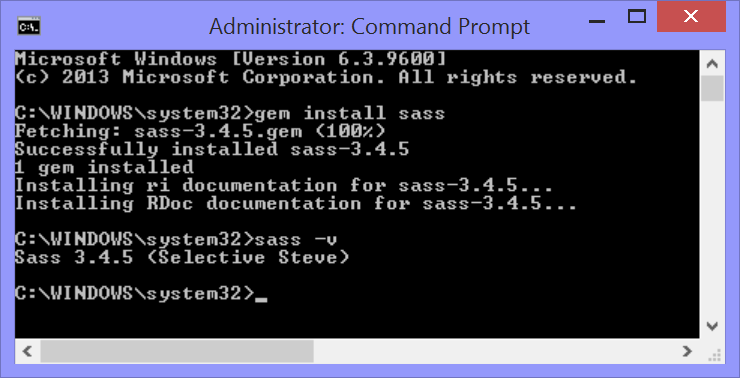
\includegraphics[width=8cm]{sassinstallation.png}
  \caption{SASS Installation}
  \label{fig:sassinstallation}
\end{figure}

\noindent
Finally in order to extend the functionality of SASS, we install the Compass css authoring library package using the following command: \texttt{gem install compass}. Similar to SASS, no explicit message indicating the success of the installation is output, but can be verified with the command: \texttt{compass -v}.

\subsection{PhpStorm Configuration}

In iCampus our SASS infrastructure, or SCSS in our case, are stored at iCampus level in \texttt{lib\_thm\_core\textbackslash scss}, at project level in \texttt{$<$Project Name$>$\textbackslash \textbackslash scss}, and lastly the compiled CSS files are stored in \texttt{$<$Project Name$>$\textbackslash $<$Project Name$>$\textbackslash media\textbackslash css}.\\
\\
The iCampus level SCSS files ensure standardized styles accross extensions. The project level styles allow for variance between individual extensions as required. To ensure that these files are not installed with the extension itself and thereby unnecessarily taking up system space these files are stored at root level in the project's repository.\\
\\
Further complicating matters, SASS files are of two basic types, signified by the beginning of the file name. Templates are complete SASS files which are normally used to generate .css files, whereas partials contain reoccurring style information used by multiple style sheets. One of the many SASS conventions regards the naming of such files. Where templates have normal names, partials begin with a ``\_" to signify them as such.\\
\\
The configuration of the PhpStorm file watchers allows for all changes made to templates in the scss folder of the project to be compiled to the its css folder. Opening a template in PhpStorm will trigger a prompt asking if you would like to create a file watcher (Figure \ref{fig:watchernotification}).\\
\\

\begin{figure}[h] 
	\centering
	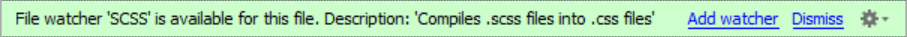
\includegraphics[width=10cm]{scsswatchernotification.png}
	\caption{File Watcher Notification}
	\label{fig:watchernotification}
\end{figure}

\noindent
To configure a file watcher either click on \texttt{Add watcher} in the notification, or navigate to \texttt{File} $>$ \texttt{Settings} then click on \texttt{File Watchers}, the \texttt{+} button on the right hand side of the interface, and finally on \texttt{SCSS} in the selection box that appears.\\
\\

\begin{figure}[h] 
	\centering
	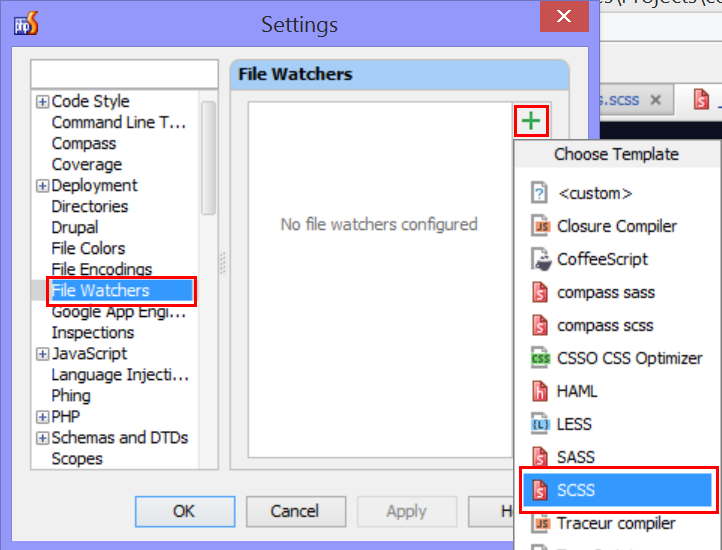
\includegraphics[width=10cm]{settingsfilewatchers.png}
	\caption{Add a New SCSS File Watcher}
	\label{fig:addscssfilewatcher}
\end{figure}

\newpage

\noindent
This brings us to the watcher edit interface seen in Figure \ref{fig:watcheredit}. This will already have default values for all fields with the exception of \texttt{Program}. Fill out the fields as described below.\\


\begin{figure}[h] 
  \centering
     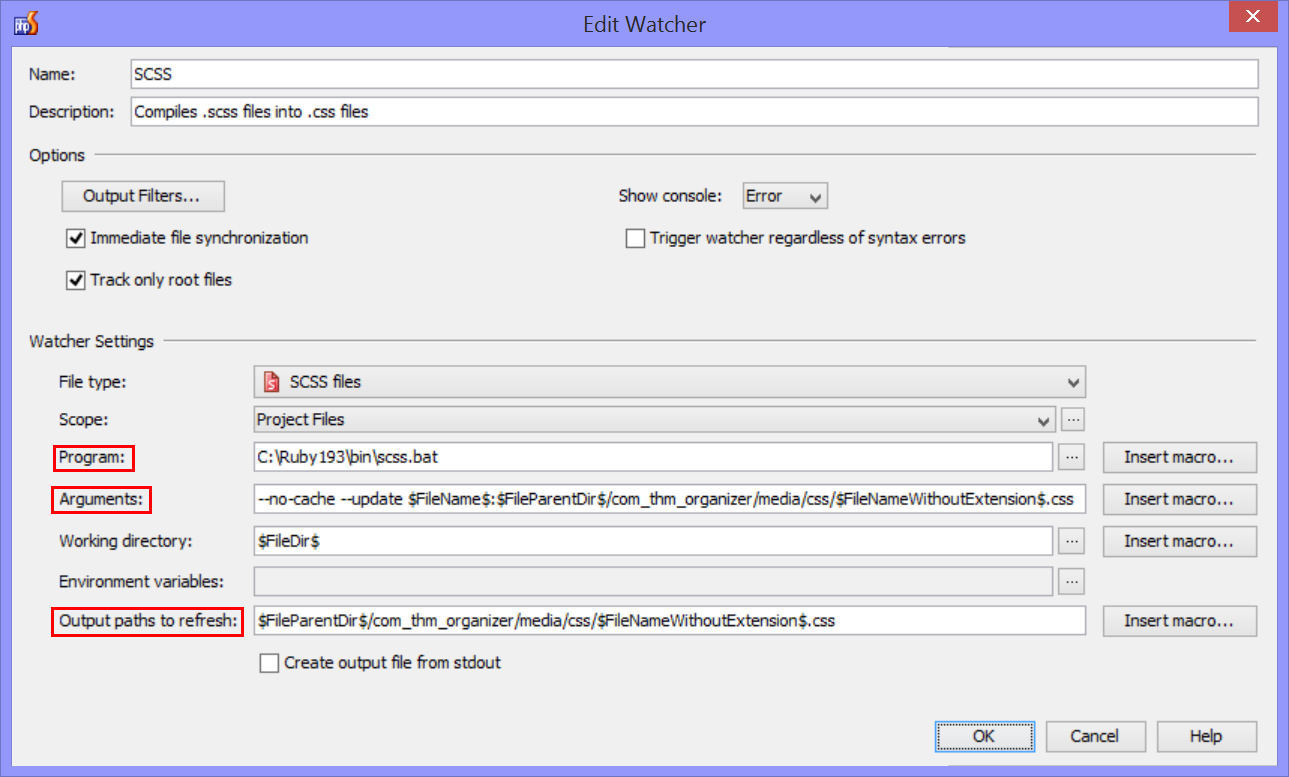
\includegraphics[width=16cm]{editwatcher.png}
  \caption{Edit File Watcher}
  \label{fig:watcheredit}
\end{figure}

\begin{description}
	\item[Program:] \texttt{$<$Ruby Installation Path$>$\textbackslash bin\textbackslash scss.bat}
	\item[Arguments:] \texttt{--no-cache --update} \newline \texttt{\$FileName\$:\$FileParentDir\$/$<$Project Name$>$/media/css/\$FileNameWithoutExtension\$.css}
	\item[Output Paths:] \texttt{\$FileParentDir\$/$<$Project Name$>$/media/css/\$FileNameWithoutExtension\$.css}
\end{description}

\noindent
Upon completion click ``OK" to save the watcher. As necessary in the \texttt{Settings} interface put a check mark in the box in front of the watcher and click ``Apply" for your changes to take effect.

\newpage

\begin{quote}
	\emph{SASS version 3.4+ automatically generates $<$File Name$>$.css.map files when used as a plugin, as well as adds comments to the .css files which reference these. While this may at some point be used for debugging purposes, I would really like to turn it off. If anyone figures out how I would be very grateful. I could not get the method explained} \href{http://sass-lang.com/documentation/file.SASS\_CHANGELOG.html#341\_22_august\_2014}{here} \emph{to work.}
\end{quote}

\noindent
The inclusion of iCampus partials from \texttt{lib\_thm\_core} is done in the scss files themselves using \texttt{@import}. If your project repository is in the same directory as \texttt{lib\_thm\_core}, the imports would constructed as follows:\\
\\
\begin{tabular}{l}
	\texttt{@import '../../lib\_thm\_core/scss/$<$Partial Name without Underscore$>$';}
\end{tabular}

\begin{quote}
	\emph{Here I would welcome any help in being able to add the directory with the partials to the SCSS path. This would reduce the import to the name of the partial to be imported.}
\end{quote}

\newpage

\section{Joomla!}

Almost all software developed by iCampus is for use within the context of the Joomla! content management system (CMS) used by the Department of Mathematics, Natural and Informatics (MNI) at the Central Hessen University of Applied Science.

\begin{quote}
	Joomla is an award-winning content management system (CMS), which enables you to build Web sites and powerful online applications. Many aspects, including its ease-of-use and extensibility, have made Joomla the most popular Web site software available. Best of all, Joomla is an open source solution that is freely available to everyone.\footnote{\url{http://www.joomla.org/about-joomla.html} Stand 27 September, 2014}
\end{quote}

\noindent
As of September 2014 iCampus is slightly between worlds as concerns Joomla!. The department's website currently still uses Joomla! version 2.5.x whereas the current Joomla! version as of 27 September, 2014 is 3.3.4.\\
\\
For feature development and bugfixes for the department's website a dump of the site will be provided for you. Otherwise development should be performed in the context ofJoomla! 3.x which can be downloaded from \href{http://www.joomla.org/download.html}{the Joomla website}. If you didn't deviate from the standard XAMPP installation you will want to extract the ZIP-Archive to the \texttt{C:\textbackslash xampp\textbackslash htdocs} directory.\\ 
\\
At this point both the Apache and the MySQL services need to be running. To do so open the XAMPP control panel, Figure \ref{fig:xamppcontrolpanel}, and click the ``Start" button next to both of these services.

\subsection{Database Creation}

For either of the development instances to function we first need to create databases for them to store their data in. To do this enter \url{http://localhost/phpmyadmin} in the address bar of your browser. This will open up the home page for your phpMyAdmin tool.\\
\\
To create a database, click on the \texttt{Databases} tab,the interface for database management will then appear. The first item on the page will be ``Create Database" under which will be an option for ``Database name" and ``Collation". Enter a name for your database and select the collation \texttt{utf8\_general\_ci} and then click \texttt{Create}. Then repeat as necessary for any further databases.\\

\begin{figure}[h] 
	\centering
	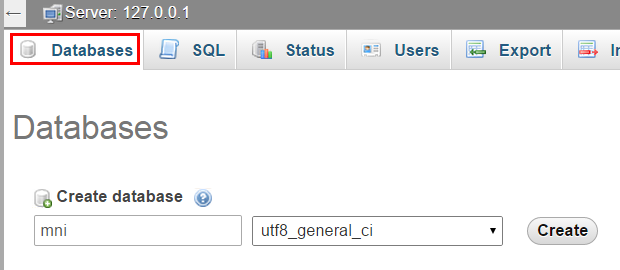
\includegraphics[width=6cm]{databasecreation.png}
	\caption{Database Creation}
	\label{fig:databasecreation}
\end{figure}

\subsection{MNI Site Development}

First we will discuss the installation of the MNI backup. If you will only be developing for Joomla! 3.x you should skip ahead to the next subsection. First extract the backup and give it an URL-friendly name such as ``mni". Next place this folder in your web directory. If you followed the default installation steps this should be located at \texttt{C:\textbackslash xampp\textbackslash htdocs}.\\
\\
Open a browser of your choosing and enter \texttt{localhost/$<$Your MNI Backup Folder$>$} in the address bar. If you renamed the backup ``mni" this would then be \url{localhost/mni}. This will automatically start the Akeeba installer. The first page shown should look like Figure \ref{fig:akeebapreinstallation}. As illustrated in the figure, we deviate from the recommended settings in one point ``Display Errors", since we changed it in Subsection \ref{subsec:phpconfig}. Should your settings not match those displayed, reconfigure your PHP settings to do so.\\

\begin{figure}[h] 
	\centering
	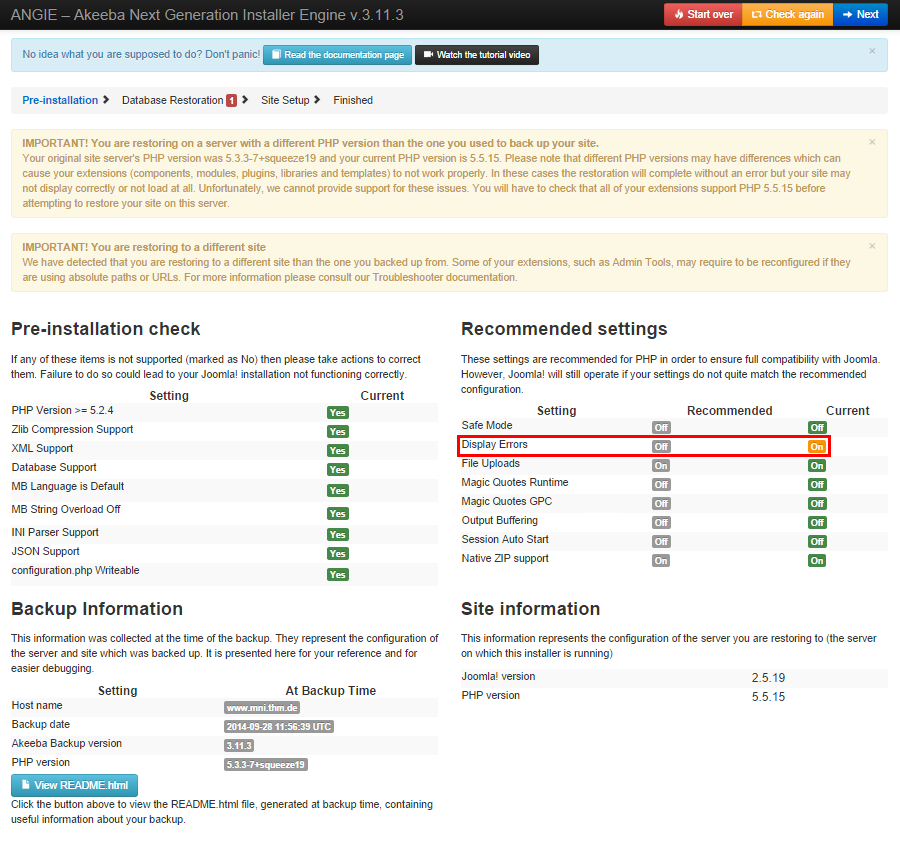
\includegraphics[width=10cm]{akeeba1.png}
	\caption{Akeeba Pre-installation}
	\label{fig:akeebapreinstallation}
\end{figure}

\noindent
Click ``$\Rightarrow$ Next". This brings us to the database restoration page seen in Figure \ref{fig:akeebadatabaserestoration}.

\newpage

\begin{figure}[h] 
	\centering
	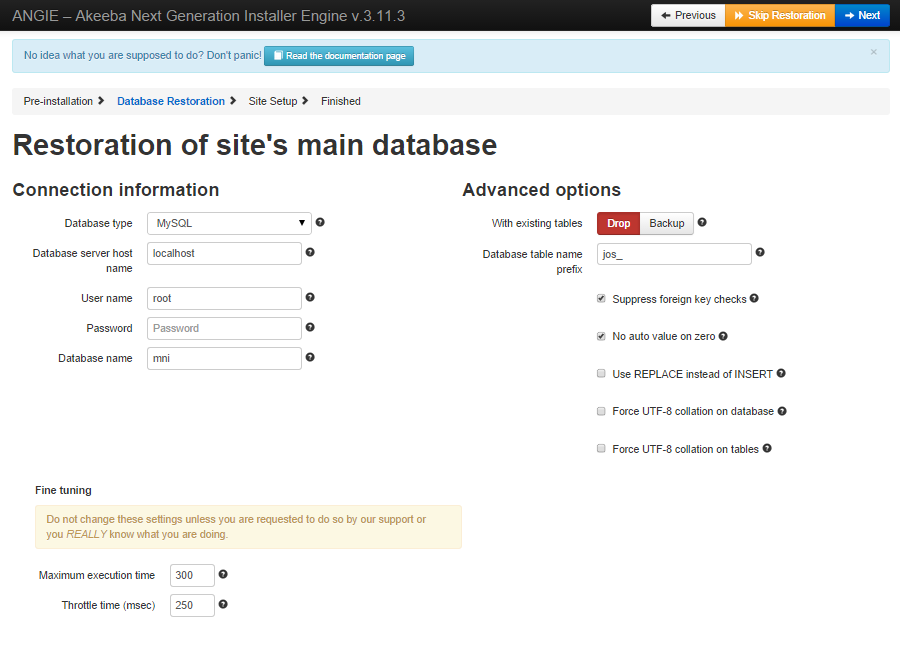
\includegraphics[width=10cm]{akeeba2.png}
	\caption{Akeeba Database Restoration}
	\label{fig:akeebadatabaserestoration}
\end{figure}

\noindent
Here use the following values:\\
\\
\begin{tabular}{l l}
	\texttt{Database type} & MySQL\\
	\texttt{Database server host name} & localhost\\
	\texttt{User name} & root\\
	\texttt{Password} & (empty, unless set)\\
	\texttt{Database name} & mni (unless named otherwise)\\
	\texttt{Maximum execution time} & 300\\\\
\end{tabular}

\noindent
Clicking ``$\Rightarrow$ Next" will trigger the restoration of the database. Then progress will then be displayed in a pop-up window. This may take up to several minutes dependent upon your computer. This brings us to the database restoration page seen in Figure \ref{fig:akeebasitesetup}.

\newpage

\begin{figure}[h] 
	\centering
	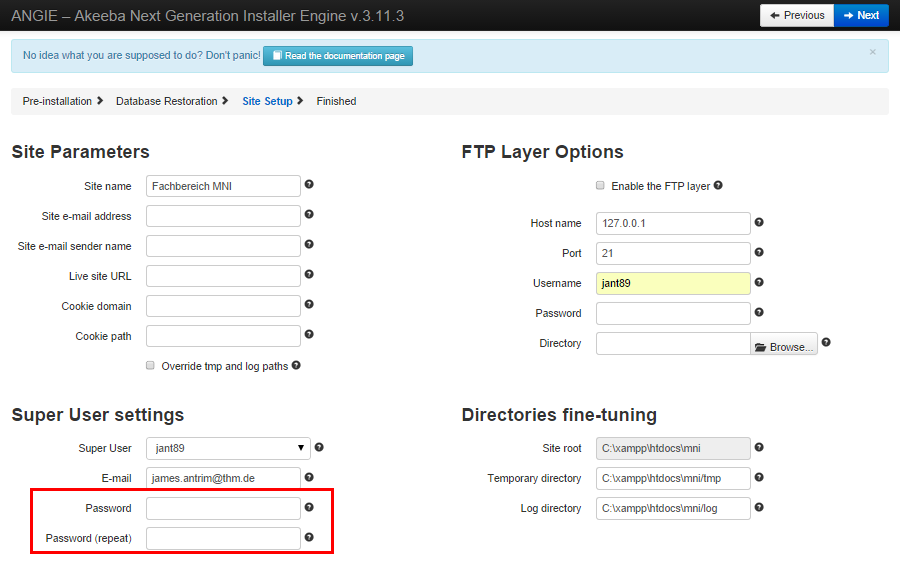
\includegraphics[width=10cm]{akeeba3.png}
	\caption{Akeeba Site Setup}
	\label{fig:akeebasitesetup}
\end{figure}

\noindent
Here you need to choose a \texttt{Super User}. The available options are the users which have super user access to the live web site. Here it is not important which user you chose, but rather that you remember which user you chose. Also important is setting a local \texttt{Password} for the chosen user, this prevents the system from validating against the data available to the CAS server. Set a new local  \texttt{Password} and repeat it in  \texttt{Password (repeat)}.\\
\\
When you click Clicking ``$\Rightarrow$ Next" you will be directed to the final confirmation page. Here you will be notified that you need to delete the \texttt{installation} directory to complete the installation. Do so by clicking on the blue button. You will then automatically be redirected to the site's frontend.

\subsection{Joomla! 3.x Development}

First abstract the archive file downloaded from \href{http://www.joomla.org/download.html}{the Joomla! website} and give it a URL friendly name such as ``j3". Next place this folder in your web directory. If you followed the default installation steps this should be located at \texttt{C:\textbackslash xampp\textbackslash htdocs}.\\
\\
Open a browser of your choosing and enter \texttt{localhost/$<$Your Joomla 3.x Folder$>$} in the address bar. If you renamed the backup ``j3" this would then be \url{localhost/j3}. This will open the main configuration page as seen in Figure \ref{fig:j3mainconfiguration}.

\newpage

\begin{figure}[h] 
	\centering
	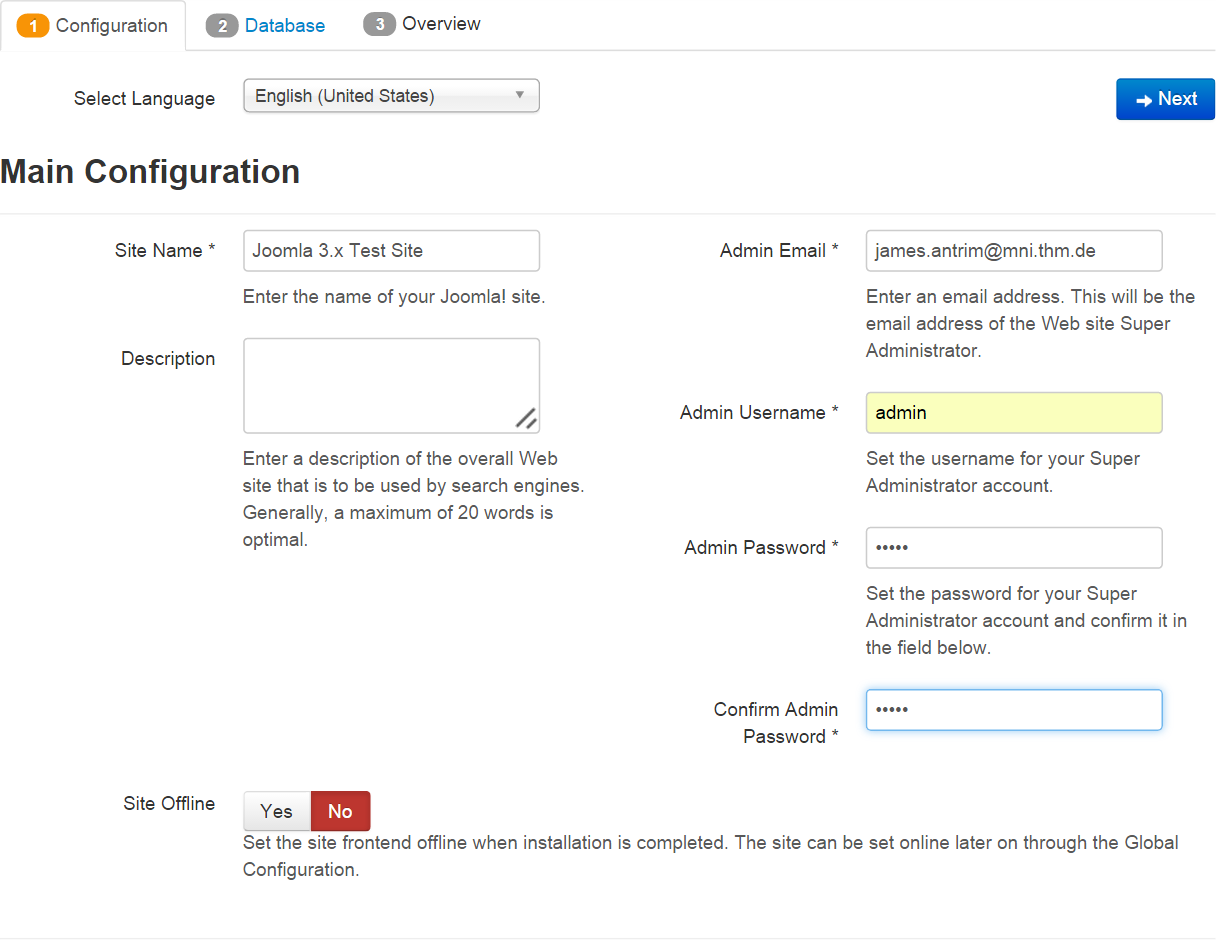
\includegraphics[width=8cm]{j3mainconfiguration.png}
	\caption{Joomla Main Configuration}
	\label{fig:j3mainconfiguration}
\end{figure}

\noindent
Here you will need to enter the \texttt{Site Name}, \texttt{Admin Email}, \texttt{Admin Username}, \texttt{Admin Password}, and \texttt{Confirm Admin Password}. Click ``$\Rightarrow$ Next" to move on to the database configuration.\\

\begin{figure}[h] 
	\centering
	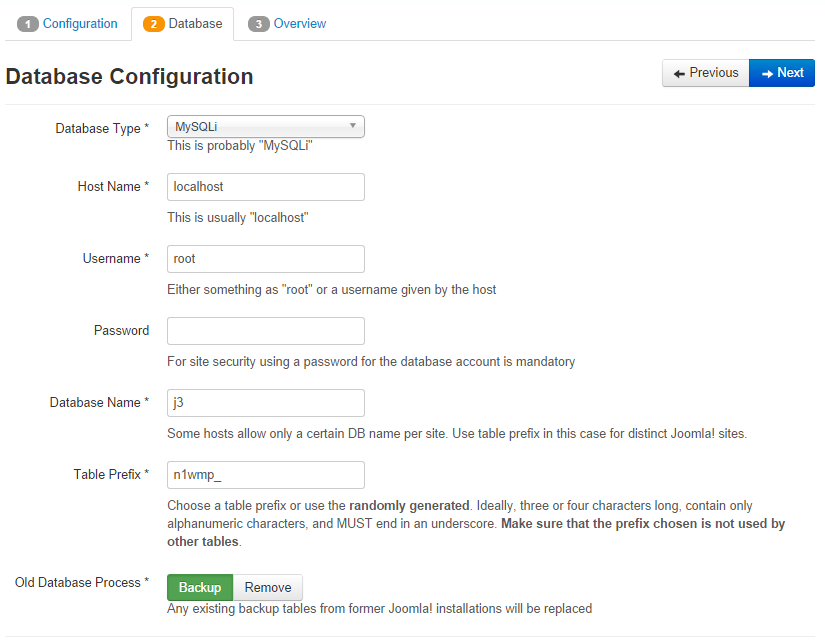
\includegraphics[width=8cm]{j3databaseconfiguration.png}
	\caption{Joomla Database Configuration}
	\label{fig:j3databaseconfiguration}
\end{figure}

\noindent
Use the following values to complete the form, then click ``$\Rightarrow$ Next" to continue on to the finalization.\\
\\
\begin{tabular}{l l}
	\texttt{Database type} & MySQLi\\
	\texttt{Host Name} & localhost\\
	\texttt{Username} & root\\
	\texttt{Password} & (empty, unless set)\\
	\texttt{Database name} & j3 (unless named otherwise)\\
\end{tabular}

\newpage

\begin{figure}[h]
	\centering
	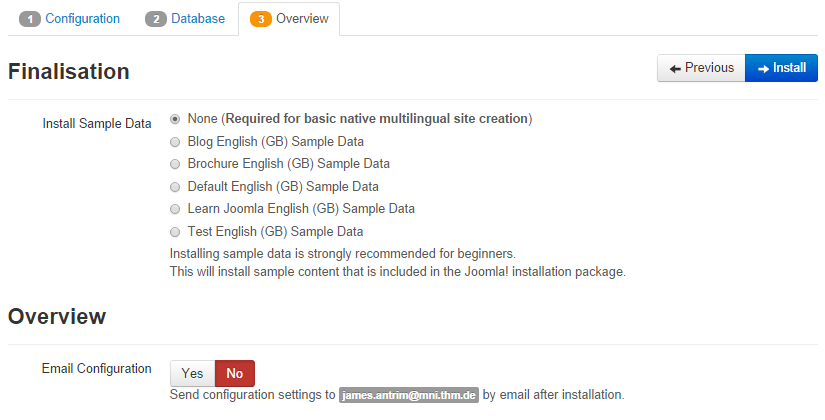
\includegraphics[width=10cm]{j3finalization.png}
	\caption{Joomla Finalization}
	\label{fig:j3finalization}
\end{figure}

\noindent
Here you can choose whether or not you wish to install sample data. Leave ``None" selected and click ``$\Rightarrow$ Install" to complete the installation. The installation will then show the progress of the database construction. When this is finished you will be told that Joomla! is installed. You should now press the orange button ``Remove installation folder" to complete the installation. You can choose to visit the frontend or backend of the site by clicking the appropriate button.

\chapter{User's Guide}

\section{Git}

\subsubsection{Create a new local branch}

\subsubsection{Add a local branch to remote}
From the repository directory in Git Bash or the PhpStorm Terminal enter:\\
\\
\begin{tabular}{l}
	\texttt{git push -u origin $<$Branch Name$>$}
\end{tabular}



\end{document}